%----------------------------------------------------------------------------------------
%	METODE
%----------------------------------------------------------------------------------------
\section*{METODE PENELITIAN}

Penelitian ini melakukan pengelompokan dengan menggunakan teknik pengelompokan dengan metode \textit{single link}. Tahapan yang dilakukan pada penelitian ini,ialah penyiapan data, ekstraksi ciri dengan \textit{k-mers}, pengelompokan sekuen DNA dengan menggunakan \textit{single link}, dan menganalisi hasil pengelompokan. Gambar \ref{fig:tahapan} menunjukan tahapan proses tersebut.

\begin{figure}[h!] % Gunakan \begin{figure*} untuk memasukkan Gambar
\centering
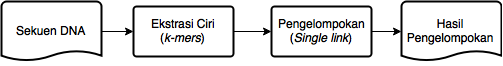
\includegraphics[width=200pt]{metode.png}
\caption{Tahapan proses penelitian}
\label{fig:tahapan}
\end{figure}

\subsection*{Penyiapan Data}

Data yang digunakan pada penelitian ini merujuk kepada penelitian \citeauthor{TAMSIN2013} (\cite*{TAMSIN2013}). Data tersebut menggunakan 50 data sekuen DNA yang terdiri dari 10 data dari genus \textit{Borellia}, 10 genus dari \textit{Streptococcus}, 10 genus dari \textit{Yersinia}, 10 genus dari \textit{Methylobacterium}, dan 10 genus dari Bacillus. Semua data diperoleh dari situs National Center of Biotechnology Information, US National Library of Medicine dalam format FASTA.

\begin{table*}[t!]
	\begin{center}
		\caption{Rencana Jadwal Penelitian}
		\label{tab:jadwal}
		\footnotesize
		\begin{tabular}{|l|c|c|c|c|c|c|c|c|c|c|c|c|c|c|c|c|c|c|c|c|}
			\hline
			\multirow{2}{*}{Kegiatan}&\multicolumn{4}{c|}{Juni}&\multicolumn{4}{c|}{Juli}&\multicolumn{4}{c|}{Agustus}&\multicolumn{4}{c|}{September}&\multicolumn{4}{c|}{Oktober}\\
			\cline{2-21}
			&1&2&3&4&1&2&3&4&1&2&3&4&1&2&3&4&1&2&3&4\\
			\hline
			Pengumpulan data dan anlisis kebutuhan sistem&\cellcolor{black}&\cellcolor{black}&\cellcolor{black}&&&&&&&&&&&&&&&&&\\
			\hline
			Perancangan dan pemodelan &&&&\cellcolor{black}&\cellcolor{black}&\cellcolor{black}&\cellcolor{black}&\cellcolor{black}&\cellcolor{black}&\cellcolor{black}&\cellcolor{black}&\cellcolor{black}&&&&&&&&\\
			\hline
			%Pemodelan data warehouse &&&&&&\cellcolor{black}&\cellcolor{black}&\cellcolor{black}&&&&&&&&&&&&\\
			%\hline
			Implementasi Sistem&&&&&&&&&\cellcolor{black}&\cellcolor{black}&\cellcolor{black}&\cellcolor{black}&&&&&&&&\\
			\hline
			Penulisan skripsi final&\cellcolor{black}&\cellcolor{black}&\cellcolor{black}&\cellcolor{black}&\cellcolor{black}&\cellcolor{black}&\cellcolor{black}&\cellcolor{black}&\cellcolor{black}&\cellcolor{black}&\cellcolor{black}&\cellcolor{black}&\cellcolor{black}&\cellcolor{black}&\cellcolor{black}&\cellcolor{black}&&&&\\
			\hline
			Seminar&&&&&&&&&&&&&&&&&\cellcolor{black}&&&\\
			\hline
		\end{tabular}
		\normalsize
	\end{center}
\end{table*}

\subsection*{Ekstraksi Ciri}
Pada tahap ini akan dilakukan ekstraksi ciri dari sekuen DNA dengan menggunakan \textit{k-mers frequency}.  Implementasi \textit{map-reduce} pada tahap ini dengan memetakan sekuen DNA ke dalam \textit{mappers}. Setiap mappers akan menghitung \textit{k-mers frequency} dari reads yang sudah dipetakan. Hasilnya akan langsung menjadi output tanpa harus melakukan \textit{reducers}. Ilustrasi proses \textit{map-reduce} untuk ekstraksi ciri dapat dilihat pada Gambar \ref{fig:kmers}.

\begin{figure}[h!]\centering % Gunakan \begin{figure*} untuk memasukkan Gambar
	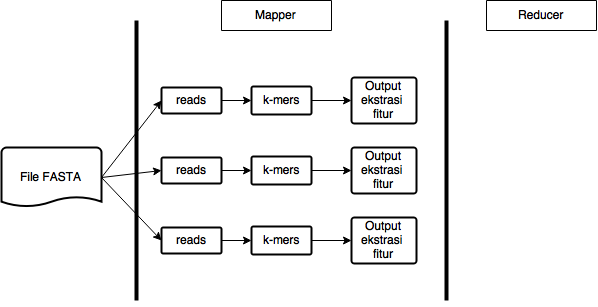
\includegraphics[width=200pt]{kmers.png}
	\caption{Illustrasi \textit{k-mers frequency} dengan model \textit{map-reduce}}
	\label{fig:kmers}
\end{figure}

\subsection*{Pengelompokan}
Ilustrasi untuk pemodelan \textit{map-reduce} dengan \textit{single link} dapat dilihat  pada Gambar \ref{fig:single}.
\begin{figure}[h!]\centering % Gunakan \begin{figure*} untuk memasukkan Gambar
	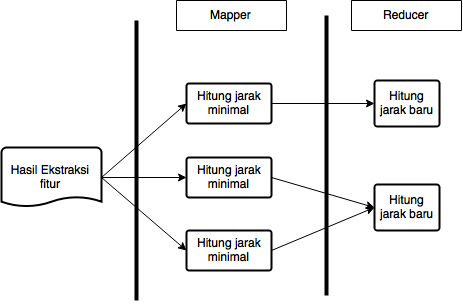
\includegraphics[width=200pt]{single.png}
	\caption{Illustrasi \textit{single link} dengan model \textit{map-reduce}}
	\label{fig:single}
\end{figure}
Ilustrasi untuk pemodelan \textit{map-reduce} dengan \textit{single link} dapat dilihat  pada Gambar \ref{fig:single}.Pada tahap ini dilakukan pengelompokan dengan menggunakan \textit{single link}. Pengelompokan dilakukan dengan data tingkat kesamaan yang didapat dari ekstraksi fitur, dimulai dengan pengelompokan menggunakan 1 data tiap genus, hingga 9 data sekuen setiap genus. Hasil dari ekstraksi akan dihitung jarak terdekatnya dan dipilih sebagai kluster, selanjutnya akan dihitung kembali jarak baru dengan memilih jarak terdekat dari kluster yang telah terpilih. 



\subsection*{Evaluasi}
Hasil dari pengelompokan \textit{single link} akan dievaluasi dengan menghitung akurasi yang diperoleh. Akurasi  akan dihitung menggunakan persamaan sebagai berikut:

\begin{equation}
Akurasi = \dfrac{\Sigma{\ data\ benar}}{\Sigma{\ jumlah\ data}}\times 100\%
\label{eq:persamaan1}
\end{equation}

\subsection*{Jadwal Kegiatan}
Penelitian ini akan dilakukan selama 4.5 bulan dengan rincian kegiatan seperti tercantum pada Tabel \ref{tab:jadwal}.

